\documentclass[10pt]{report}
\setlength{\parindent}{10pt}
\setlength{\parskip}{0,9em}
\usepackage{indentfirst}
\usepackage[margin=1in, paperwidth=8.5in, paperheight=11in]{geometry}
\usepackage{hyperref}
\usepackage[utf8]{inputenc}
\usepackage[T1]{fontenc}
\usepackage{polski}
\usepackage[polish]{babel}
\usepackage{lmodern}
\usepackage{multirow}
\usepackage{amsfonts}
\usepackage{graphicx}
\usepackage{placeins}
\usepackage{courier}
\usepackage{listings}
\usepackage{color}
\definecolor{codegreen}{rgb}{0,0.6,0}
\definecolor{codeorange}{rgb}{1,0.54,0}
\lstdefinestyle{CppStyle}{
  belowcaptionskip=1\baselineskip,
  breakatwhitespace=false,
  breaklines=true,
  captionpos=b, 
  frame=below,
  aboveskip=20pt,
  belowskip = 10pt,
  language=C++,
  showstringspaces=false,
  showspaces=false,
  numbersep=5pt,
  numbers=left,  
  numberstyle=\small,
  commentstyle=\color{codegreen},
  keywordstyle=\color{magenta},
  stringstyle=\color{codeorange},
  basicstyle=\small\ttfamily,
}
\lstset{escapechar=@,style=CppStyle}

\title{Projekt realizowany na zajęcia 'inżynierii e-systemów w technologii JAVA'}
\author{
	\textit{\textbf{Autor:} Sebastian Wilgosz}\\
}
 
\makeatletter
\renewcommand{\maketitle}{
\begin{titlepage}
    \begin{center}
        \vspace*{1cm}
        \large{Informatyka, Wydział Elektroniki Politechniki Wrocławskiej}\par
        \vspace*{3,5cm}
        \LARGE\textbf{Edytor map 3D}\par
        \vspace {10mm}
        \large\textbf{\@title}\par
        \vspace{5cm}
    
    	\large{\@author}\par   	  		
    	\vspace {10mm}
    	
    	\large\textbf{\textit{Prowadzący:}}\\
       	\large\textbf{dr inż. Tomasz Walkowiak}\par
        \vspace{3cm}
        \small \@date
    \end{center}
\end{titlepage}
}
\makeatother

\begin{document}
\maketitle
\tableofcontents
\newpage

\chapter{Cel i zakres projektu}
\section{Zakres projektu}
Niniejszy projekt będzie zawierał opis techniczny i specyfikację kroków, wykorzystania narzędzi niezbędnych do stworzenia aplikacji w środowisku \textbf{Java IEE} .
Projekt będzie uwzględniał następujące etapy : 
\begin{enumerate}
\item{Analiza i Specyfikacja}
\item{Projektowanie}
\item{Implementacja}
\item{Testy}
\item{Ocena i Optymalizacja}
\end{enumerate}

\section{Cel projektu}
Celem projektu jest wykonanie aplikacji serwerowej. 
Aplikacja będzie budowana w oparciu o technologię \textbf{Java IEE}.
Sam sposób wdrożenia programu jak i jego zadania wraz z implementacją będą przebiegały wedle przedstawionego pomysłu, który został wstępnie zaakceptowany przez prowadzącego kurs.
Projekt ma na celu zapoznać Studentów specjalizacji Inżynieria Internetowa z procesem 
budowania oprogramowania obecnie stosowanego w świecie aplikacji serwerowych.
Projekt dodatkowo dzięki wybranemu tematowi pomoże zgłębić technologie strony klienckiej
takie jak \textbf{WebGL} i \textbf{JavaScript}

\chapter{Analiza i Specyfikacja}
\section{Opis słowny zadania}
Celem naszej pracy projektowej jest stworzenie aplikacji zdolnej do tworzenia i zarządzania mapkami 3d terenu.
Niniejsza aplikacja serwerowa ma za zadanie wspomagać tworzenia ciekawych wizualizacji terenu dla osób zajmujących się hobbystycznie jak i zawodowo kartografią.
Tworzone przez użytkowników prace można będzie łączyć, zlecać wykonanie na nich danych obliczeń w celu wykorzystania ich w danym problemie.
Nasz serwis z aplikacją nazwaliśmy \\\textbf{\textit{"Avalanche"}} \textit{[eng. lawina]}, w dalszej części projektowania i założeń podamy bliższe szczegóły naszych kroków projektowych.
Aplikację w przyszłości może uda rozwinąć się do dużo ciekawszych zastosowań.
\section{Specyfikacja wymagań funkcjonalnych}
\boxy{Prezentacja bazy punktów w formie mapy}{Jest to główna funkcja tej aplikacji, ma ona za zadnie z zadanego zbioru danych generować podgląd danego terenu w formie obrotowej mapki w przestrzeni trójwymiarowej.}
\newpage
\boxy{Oddzielne sesje dla każdego użytkownika}{Ponieważ aplikacja będzie zawierała w sobie proces tworzenia jakiegoś elementu terenu niezbędne będzie wyodrębnienie pojedynczych działań na aplikacji w formie sesji użytkowników, którzy swoje gotowe mapki będą mogli dzięki powiązaniu z kontem przechowywać w zdalnej przestrzeni dyskowej} 
\boxy{Wczytywanie mapek z pliku}{Poza wczytywaniem mapek z bazy serwera możliwe będzie wczytywanie wcześniej zapisanych mapek z pliku. Funkcjonalność taka będzie przydatna gdy użytkownik po wykasowaniu maki bądź usunięciu konta, chciałby odtworzyć swoje prace}
\boxy{Łączenie kilku prac w jedną}{Serwer będzie mógł według kilku definiowanych zasad łączyć kilka zasobów w jedną wspólną mapę, taka funkcjonalność będzie przydatna przy tworzeniu pracy opartej na wkładzie kilku użytkowników}
\boxy{Generacja map}{Generacja mapek na podstawie już istniejącej z podanymi zasadami zmiany oraz tworzenie totalnie losowej mapy}
\boxy{Zapisywanie prac na serwerze}{Każda stworzona mapka będzie dostępna niezależnie od miejsca i sprzętu użytkownika poprzez interfejs webowy dostępny w przeglądarce internetowej}
\boxy{Eksport gotowych prac do określonych formatów}{Każdą z gotowych prac będzie można wyeksportować do formatu możliwego do użytku w celu prezentacji/wizualizacji z założenia są to formaty 
\textbf{*.pdf *.jpeg}.}


\section{Specyfikacja wymagań niefunkcjonalnych}
\setcounter{boxCount}{1}
\boxy{Przejrzysty interfejs webowy}{Wymaganiem jest by aplikacja była nie przeładowana dodatkami i prosta w obsłudze dla osób nie posiadających zdolności programistycznych}
\boxy{Szybkość i oszczędność łącza}{Aplikacja powinna większość pracy wykonywać bez potrzeby generowania zbędnego ruchu sieciowego co pomoże zaoszczędzić zasoby klienta}
\boxy{Multiplatformowość}{Aplikacja powinna generować taki sam rezultat niezależnie od platformy sprzętowej klienta}
\boxy{Baza danych MySQL}{Zasób danych powinien być przechowywany na łatwej w obsłudze i bezpłatnej dystrybucji bazy danych, takiej jak np. \textbf{MySQL}}
\boxy{Dane o twórcach jak i projekcie}{Aplikacja będzie zawierała informacje o okolicznościach w jakich powstała i dla jakich celów}
\boxy{Model MVC}{Aplikacja będzie opierać się na modelu MVC}
\boxy{Dokumentacja}{Przebieg procesu powstawania jak i opis funkcjonalności i sposób wykorzystania poszczególnych funkcji będzie zawarty w dokumentacji projektu}
\chapter{Instrukcja użytkownika}

\section{Wersja Pordukcyjna}
Wersja produkcyjna aplikacji jest uruchomiona na serwerze heroku, pod adresem \url{http://terrain-editor.herokuapp.com}{http://terrain-editor.herokuapp.com}

Pierwsze uruchomienie wymaga uruchomienia serwera, który przechodzi w stan uśpienia po godzinie braku aktywności ze strony użytkowników w celu oszczędności zasobów. Z tego powodu po wpisaniu adresu w przeglądarce internetowej po raz pierwszy, należy zaczekać nieco dłużej niż w przypadku kolejnych zapytań do serwera.

\subsection{Logowanie i rejestracja}
Aby mieć dostęp do wszystkich funkcji aplikacji, należy się zalogować, lub zarejestrować nowego użytkownika.

Ze względu na przeznaczenie projektu do celów edukacyjnych, postanowiłem nie walidować adresów email pod kątem prawdziwości, dlatego dopuszczalne do rejestracji są fałszywe adresy, pod warunkiem że zachowany zostanie poprawny format.

W wersji pokazowej zarejestrowany został użytkownik:
\textbf{email:} test.user@example.com
\textbf{hasło:} password

\FloatBarrier
 	\begin{figure}[ht]
        \centering
        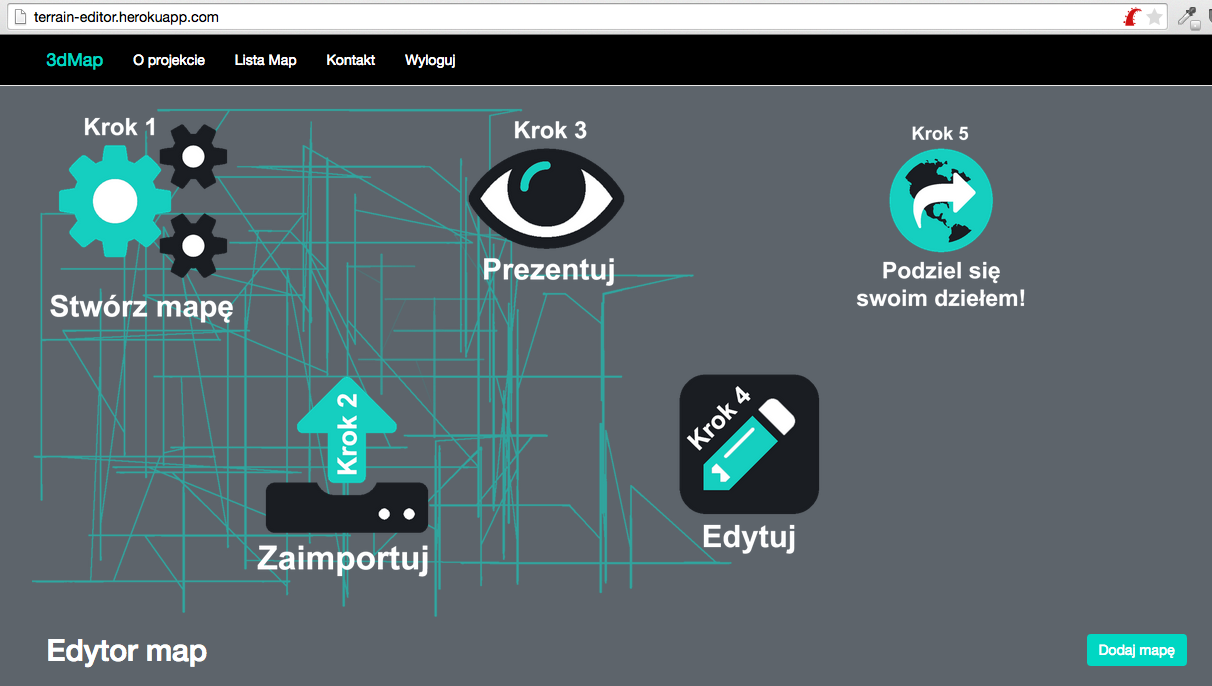
\includegraphics[width=0.90\textwidth,height=0.46\textheight]{img/home.png}
	\caption{Strona główna aplikacji}
        \label{rys:screen_home}
    \end{figure}
\FloatBarrier
	
\subsection{Kontrola dostępu}

Wykorzystanie sesji logowania pozwoliło na ograniczenie praw dla użytkowników niezalogowanych, jak i dla zalogowanych.

\begin{itemize}
\item Użytkownicy niezalogowani mogą:
	\subitem Przeglądać mapy
	\subitem Logować się, i rejestrować
	\subitem Wysyłać emaile kontaktowe
			
\item Użytkownicy zalogowani mogą:
	\subitem Wykonywać wszystkie akcje niezalogowanych użytkowników z wyjątkiem rejestracji i logowania.
	\subitem Dodawać mapy
	\subitem Edytować swoje mapy
\end{itemize}

W przypadku próby wykonania akcji zabronionej, użytkownik niezalogowany jest przekierowywany do ekranu logowania, zaś zalogowany użytkownik do strony głównej.

Na górze ekranu pojawi się wiadomość o braku uprawnień do wykonania danej akcji.

\FloatBarrier
 	\begin{figure}[ht]
        \centering
        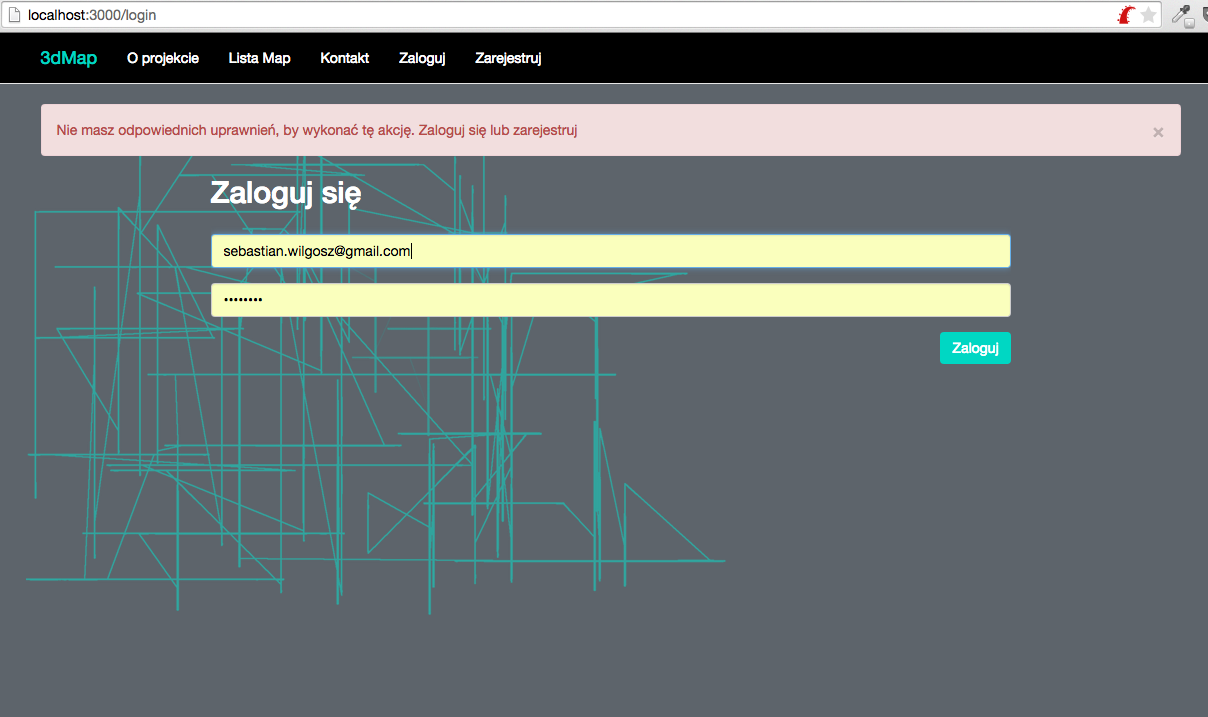
\includegraphics[width=0.90\textwidth,height=0.46\textheight]{img/no_access.png}
	\caption{Próba wykonania akcji zabronionej}
        \label{rys:screen_no_access}
    \end{figure}
\FloatBarrier

\subsection{Wysyłanie emaili}

Aplikacja umożliwia wysłanie wiadomości kontaktowej do administratorów systemu. Z powodu udostępnienia aplikacji online, postanowiłem wyłączyć funkcję wysyłania maili na rzeczywistą skrzynkę odbiorczą. Zamiast tego zintegrowałem projekt z aplikacją \textit{Mailtrap}, która przechwytuje wszystkie emaile wysyłane z konta pocztowego. W celu rekonfiguracji konta, zobacz sekcję: \ref{dev_mailer}.

\subsection{Dodawanie mapy z pliku}

Dodawanie nowych map jest dostępne wyłącznie dla zalogowanych użytkowników. Jeżeli chcesz dodać mapę, będąc zalogowanym kliknij w przycisk na stronie głównej, liście map albo stornie pojedynczej mapy.

\FloatBarrier
 	\begin{figure}[ht]
        \centering
        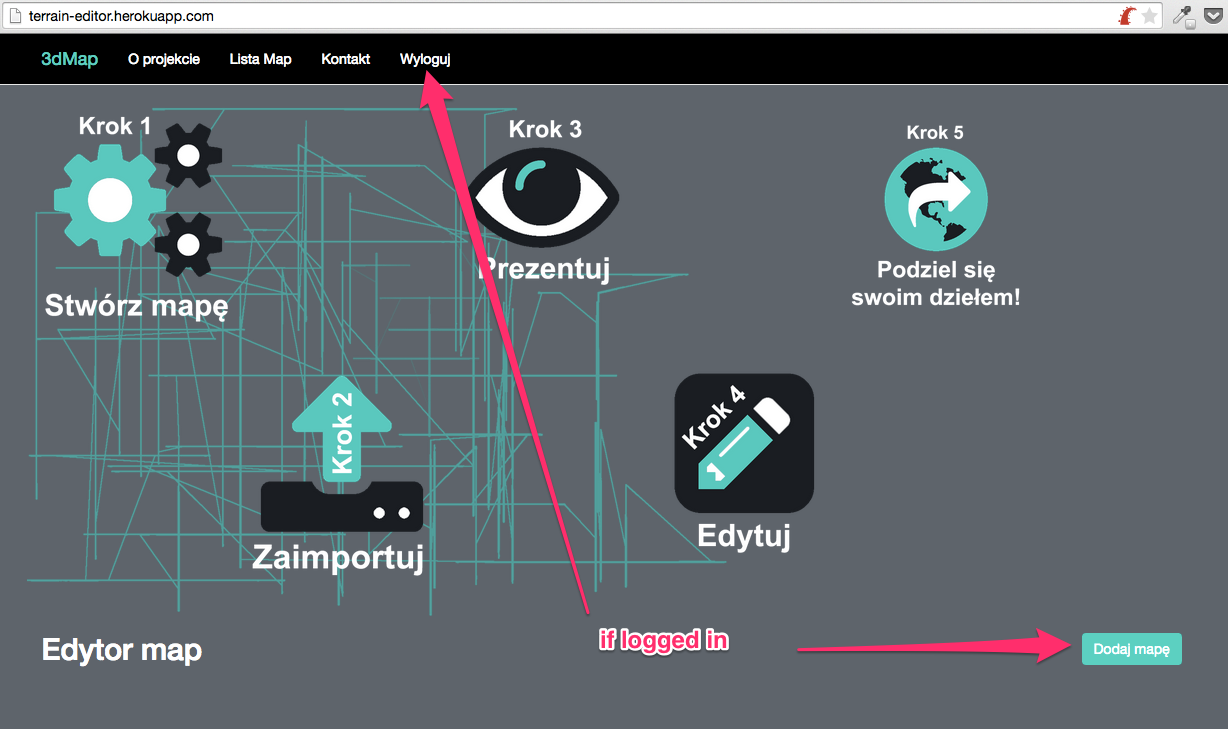
\includegraphics[width=0.90\textwidth,height=0.46\textheight]{img/add_map1.png}
	\caption{Dodawanie mapy, krok 1}
        \label{rys:screen_add_map1}
    \end{figure}
\FloatBarrier

Po kliknięciu w przycisk pojawi się formularz dodawania nowej mapy. Schemat należy wczytać z odpowiednio sformatowanego pliku tekstowego.

Plik powinien mieć następujący format:

\begin{table}[h]
	\centering
	\begin{tabular}{|l|l|l|l|l|l|}
		Source X & Source Y & Source Z & Target X & Target Y & Target Z \\ \hline
	\end{tabular}
	\caption{Format pliku z danymi mapy do importu.}
	\label{tab:file_format}
\end{table}

Lub powinine być plikiem tekstowym, w którym każda linia odpowiada kolejnemu wierszowi, zaś komórki są oddzielone średnikiem (";").

W celach prezentacyjnych do repozytorium zostały dołączone przykładowe pliki z danymi do zaimportowania w katalogu \textit{app/assets/csv/*}.
	
\section{Wersja lokalna}

ubuntu/reverse

\subsection{Wysyłanie emaili}
\label{dev_mailer}
\chapter{Podsumowanie}
\label{summary}

\textbf{Projekt był początkowo z przeznaczony dla dwóch osób}. Niestety, dwa tygodnie przed oddaniem drugi członek zespołu zrezygnował z kontynuowania nauki, nie dołączając żadnego wkładu ze swojej strony.

Z tego powodu nie udało mi się wykonać wszystkich funkcji, jakie zostały założone w specyfikacji początkowej.

\section{Wykonane założenia}

\begin{enumerate}
\item \textbf{Wysyłanie emaili kontaktowych} - użytkownicy powinni mieć możliwość wysyłania maili do administratorów w razie problemów.

  \item \textbf{Prezentacja bazy punktów w formie mapy} - Jest to główna funkcja tej aplikacji, ma ona za zadnie z zadanego zbioru danych generować podgląd danego terenu w formie obrotowej mapki w przestrzeni trójwymiarowej.

  \item \textbf{Oddzielne sesje dla każdego użytkownika} - Ponieważ aplikacja będzie zawierała w sobie proces tworzenia jakiegoś elementu terenu niezbędne będzie wyodrębnienie pojedynczych działań aplikacji w formie sesji użytkowników, którzy swoje gotowe mapy będą mogli dzięki powiązaniu z kontem przechowywać w zdalnej przestrzeni dyskowej
  
  \item \textbf{Wczytywanie map z pliku} - Poza wczytywaniem map z bazy serwera możliwe będzie wczytywanie wcześniej zapisanych map z pliku. Funkcjonalność taka będzie przydatna gdy użytkownik po wykasowaniu mapy bądź usunięciu konta, chciałby odtworzyć swoje prace.
  
  \item \textbf{Generacja map} - Generacja map na podstawie już istniejącej z podanymi zasadami zmiany oraz tworzenie totalnie losowej mapy
  
  \item \textbf{Zapisywanie prac na serwerze} - Każda stworzona mapa będzie dostępna niezależnie od miejsca i sprzętu użytkownika poprzez interfejs webowy dostępny w przeglądarce internetowej
  
  \item \textbf{Przejrzysty interfejs webowy} - Wymaganiem jest by aplikacja była nie przeładowana dodatkami i prosta w obsłudze dla osób nie posiadających zdolności programistycznych

  \item \textbf{Szybkość i oszczędność łącza} - Aplikacja powinna większość pracy wykonywać bez potrzeby generowania zbędnego ruchu sieciowego co pomoże zaoszczędzić zasoby klienta

  \item \textbf{Multiplatformowość} - Aplikacja powinna generować taki sam rezultat niezależnie od platformy sprzętowej klienta

  \item \textbf{Baza danych MySQL} - Zasób danych powinien być przechowywany na łatwej w obsłudze i bezpłatnej dystrybucji bazy danych, takiej jak np. \textbf{MySQL}
  
  \item \textbf{Dane o twórcach jak i projekcie} - Aplikacja będzie zawierała informacje o okolicznościach w jakich powstała i dla jakich celów
  
  \item \textbf{Model MVC} - Aplikacja opiera się na modelu MVC
  
  \item \textbf{Dokumentacja} - Przebieg procesu powstawania jak i opis funkcjonalności i sposób wykorzystania poszczególnych funkcji będzie zawarty w dokumentacji projektu
\end{enumerate}



\section{Niewykonane założenia}

\begin{enumerate}
  \item{Eksport gotowych prac do określonych formatów}{Każdą z gotowych prac będzie można wyeksportować do formatu możliwego do użytku w celu prezentacji/wizualizacji z założenia są to formaty \textbf{*.pdf *.jpeg}.}

  \item \textbf{Łączenie kilku prac w jedną} - Serwer będzie mógł według kilku definiowanych zasad łączyć kilka zasobów w jedną wspólną mapę, taka funkcjonalność będzie przydatna przy tworzeniu pracy opartej na wkładzie kilku użytkowników
  
\end{enumerate}
\FloatBarrier
	%bibliografia
\begin{thebibliography}{1}
	\bibitem{wilgoszpl_ror_installation} Instalacja Ruby On Rails na Ubuntu, Sebastian Wilgosz 2013, \url{http://blog.wilgosz.pl/pl/posts/ruby-on-rails/ruby-on-rails-instalacja-ubuntu-12-04}
\end{thebibliography}

\end{document}
